\section{MiniNet}
\subsection{Router vs Switch}
A switch is a device that operates at the data link layer (2). 
It uses the MAC addresses of devices to forward network traffic between them
within the same LAN.\\
A router, on the other hand, operates at the IP layer (3).
It uses IP addresses to forward network traffic between devices that are in
different LAN's.
\subsection{}
The output is:\\
\begin{verbatim}
    mininet> h1 ifconfig
    h1-eth0   Link encap:Ethernet  HWaddr d6:e9:4b:ad:4c:62  
            inet addr:10.0.0.1  Bcast:10.255.255.255  Mask:255.0.0.0
            inet6 addr: fe80::d4e9:4bff:fead:4c62/64 Scope:Link
            UP BROADCAST RUNNING MULTICAST  MTU:1500  Metric:1
            RX packets:7 errors:0 dropped:0 overruns:0 frame:0
            TX packets:8 errors:0 dropped:0 overruns:0 carrier:0
            collisions:0 txqueuelen:1000 
            RX bytes:558 (558.0 B)  TX bytes:648 (648.0 B)

    lo        Link encap:Local Loopback  
            inet addr:127.0.0.1  Mask:255.0.0.0
            inet6 addr: ::1/128 Scope:Host
            UP LOOPBACK RUNNING  MTU:65536  Metric:1
            RX packets:0 errors:0 dropped:0 overruns:0 frame:0
            TX packets:0 errors:0 dropped:0 overruns:0 carrier:0
            collisions:0 txqueuelen:0 
            RX bytes:0 (0.0 B)  TX bytes:0 (0.0 B)
\end{verbatim}
\begin{enumerate}
    \item The MAC is: \texttt{d6:e9:4b:ad:4c:62}.
    \item The IP is: \texttt{10.0.0.1}, subnet mask: \texttt{255.0.0.0},
    so there are 24 bits to specify different hosts in the subnet meaning there can be up to $2^{24}$ hosts in it.
    \item The IPv6 address is \texttt{fe80::d4e9:4bff:fead:4c62/64}.
    \item The MTU is 1500 (bytes).
    \item \texttt{txqueuelen} refers to the length of the transmission queue of this interface,
    which is a buffer that holds packets that are waiting to be transmitted by the interface.
\end{enumerate}
\subsection{}
A loopback interface is an interface that connects the host to itself.\\
These interfaces are useful for many things; among the most important ones I can think of
are for platform-independent IPC, and for testing network services (for example I can run \texttt{ssh localhost}
before attempting to log in somewhere else to make sure my ssh client is working properly).\\
The associated IP address \texttt{127.0.0.1} is a special address dedicated to loopback adapters.
\subsection{}
The output is almost identical - but the two have different IP and MAC addresses.
They are both in a private network \texttt{10.*.*.*} - (which we know is the same private network).
This also means that the first 8 bits of their IPv4 address match (in-fact the first 30 bits do,
but that is more of a coincident).

\subsection{}
We have used the following commands to configure the routers:
\begin{itemize}
    \item For R1: '\texttt{ip route 2.2.2.0/24 192.168.1.2}'
    \item For R2: '\texttt{ip route 3.3.3.0/24 192.168.2.2}'
    \item For R3: '\texttt{ip route 192.168.1.0/24 192.168.2.1}'
\end{itemize}
\begin{center}
    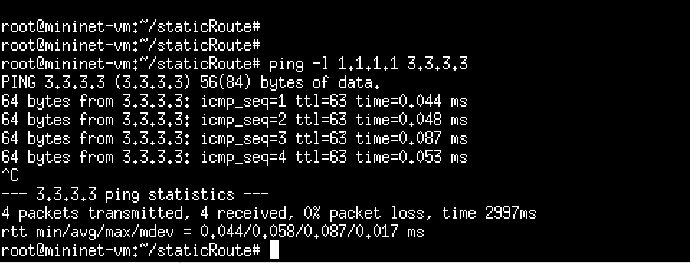
\includegraphics[width=1.2 \textwidth]{resources/mn1.png}\centering
\end{center}

\subsection{}
The main disadvantage of using static routing is that it needs to be manually defined
by the network administrator, which can be very time consuming and unscalable,
moreover - static routing is also less resilient to router crashes.

\subsection{}
In the '\texttt{count to infinity}' 
The '\texttt{count to infinity}' problem is a problem in which the router loses the link
to a specific destination before it can update its neighbors. It receives a message from
one of them that there is an alternate route that is much shorter than the one to the
destination that was lost. However, the alternate route actually passes through the first
router, which does not exist because one of the links has failed. The result is that both
routers will update each other with incorrect routes to a specific destination and packets
that will arrive at these routers in order to reach the destination will be stuck.
The process will continue until the routes that the routers exchange between them are less
efficient than another route (since their cost only increases).

\subsection{}
The mechanism is an addition to split horizon,
so that instead of a router receiving reports from routers that may be using routes
through it, it will receive them and define their use as an infinite cost, thus preventing
the sending router from being poisoned.

\subsection{}
Triggered updates is a protocol designed to try to speed up the solution of the count to
infinity problem. In cases where the "misleading cycle" is more than two routers,
split horizon will not help us. The way to do this is to send update messages as soon as an
update message is received, even if it is not the time when we (as a router) are supposed to
send update messages, and thus speed up the convergence of the count-to-infinity problem and
accelerate the network's recovery.

\subsection{}
The protocol is restricted to networks where the longest path requires no more than 15 hops.
The protocol relies on "counting to infinity" to address certain uncommon scenarios,
which can lead to lengthy convergence periods. Additionally, the protocol utilizes "hop count" exclusively and disregards other real-time parameters,
such as measured delay, reliability, or load.
\subsection{}
Every datagram has a specific purpose, and the command field is used as a header to the datagram,
where its purpose is mentioned. This includes types such as response, 
request, trace off, trace on, and reserved.
\subsection{}
Based on our count, it takes an average of \texttt{20} seconds between each response.
\subsection{}
The message is sent via UDP, on port \texttt{17}.
\subsection{}
The IP address of the destination is \texttt{224.0.0.9}, whats important about this 
address is that it is used by the RIP for multicast.
\subsection{}
The important detail that the responce message contains is the Metric,
Which represents the hop count. That is the number of router that a message needs to go through
to reach its destination.
\begin{center}
    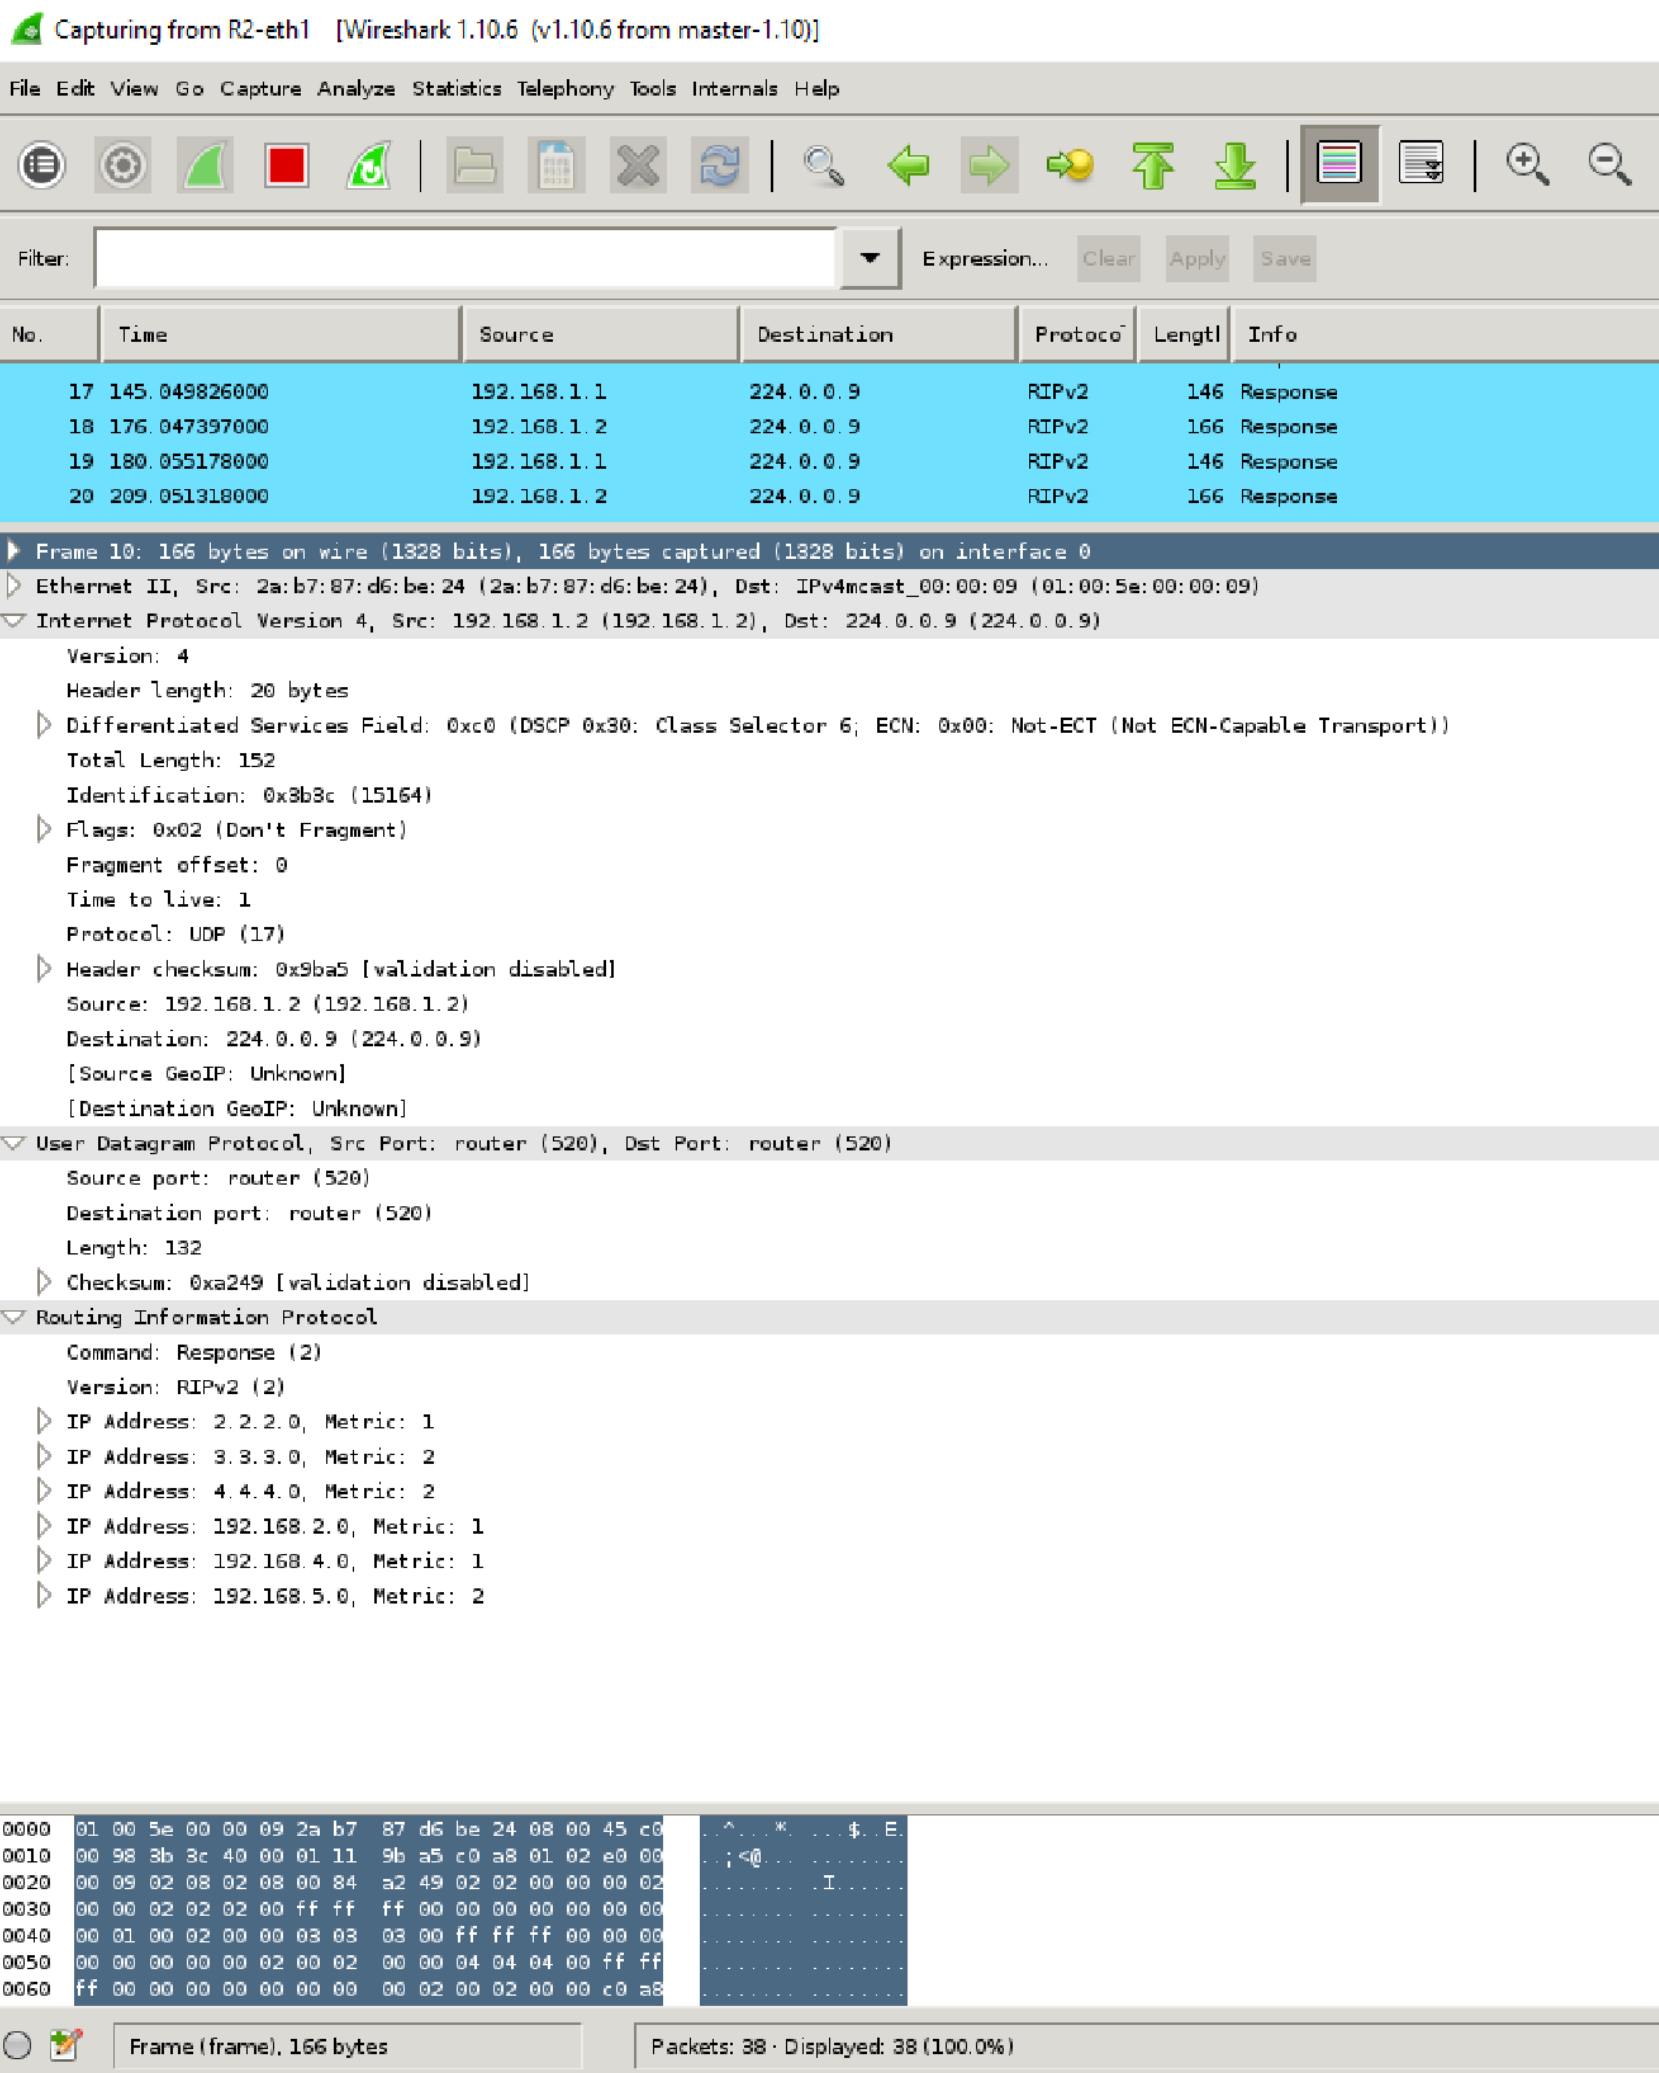
\includegraphics[width=1.2 \textwidth]{resources/mn2.png}\centering
\end{center}
\subsection{}
In our tests, the infinity metric was 16, this should be relatively long compared to the
other routes in the network (there shouldn't be any other router with longer route)

\subsection{}
Shortly after the link went down, the other nodes (routers) realized that they had a better way to reach node 4.
Thanks to the Triggered Updates mechanism. They send their own responses with updates about better paths as soon
as they realized the previous path was no longer the better one.
\begin{center}
    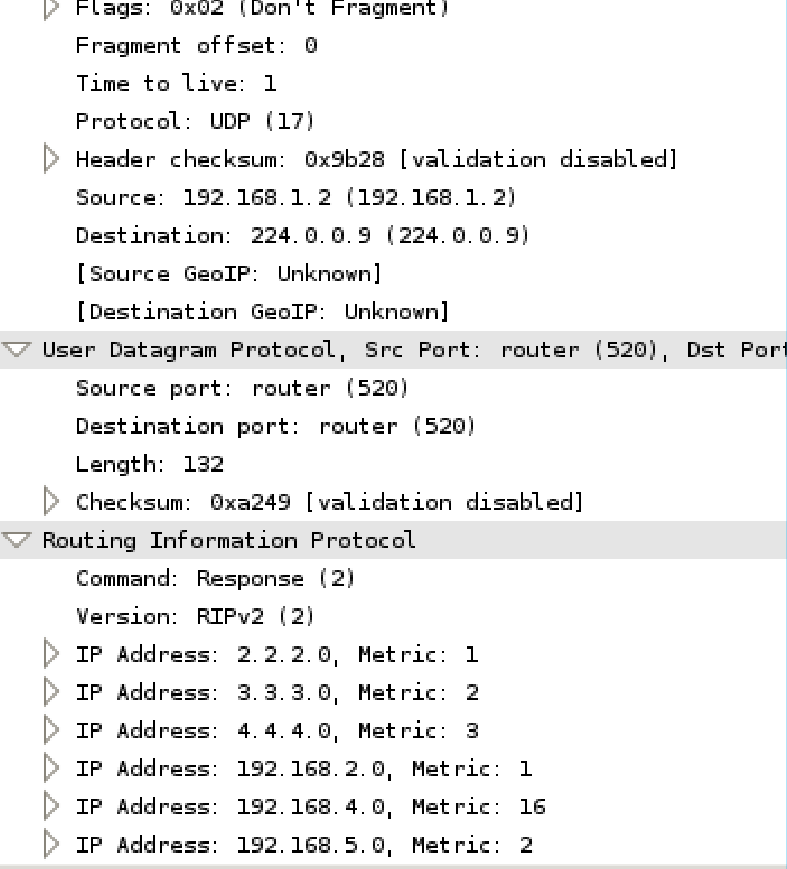
\includegraphics[width=1 \textwidth]{resources/mn3.png}\centering
\end{center}